\documentclass[12pt]{article}

\usepackage{geometry}
\geometry{a4paper, left=1in, right=1in, top=1in, bottom=1in}
\usepackage{amsmath}
\usepackage{amsmath,amsfonts,amssymb}
\usepackage{graphicx}
\usepackage{enumitem}
\usepackage{titlesec}
\usepackage{fancyhdr}
\usepackage{hyperref}
\usepackage{floatrow}
\usepackage{geometry}
\usepackage{fancyhdr}
\usepackage{empheq}
\usepackage[svgnames]{xcolor}
\usepackage{xpatch}

\makeatletter
\newcommand{\colorboxed}[1]{\fcolorbox{Black}{White}{\m@th$\displaystyle#1$}}
\xpatchcmd{\@Aboxed}{\boxed}{\colorboxed}{}{}
\makeatother

\title{{\bf CS663 Assignment 1}}
\author{Saksham Rathi, Kavya Gupta, Shravan Srinivasa Raghavan}
\date{August 2024}
\begin{document}
\maketitle
\clearpage
\tableofcontents
\clearpage
\section*{Question 5}
\addcontentsline{toc}{section}{Question 5}
    \vspace{-10pt}
    
    \textbf{(a)} The code is in \verb|../code/myMainScript.m| and the rotated image is \verb|images/T2_rotated.jpg|. \newline
    \textbf{(b)} The code is in \verb|../code/myMainScript.m|. \newline
    \textbf{(c)} Here are the graphs:-
    
    \vspace{-13pt}
    
    \begin{figure}[H]
        \centering
        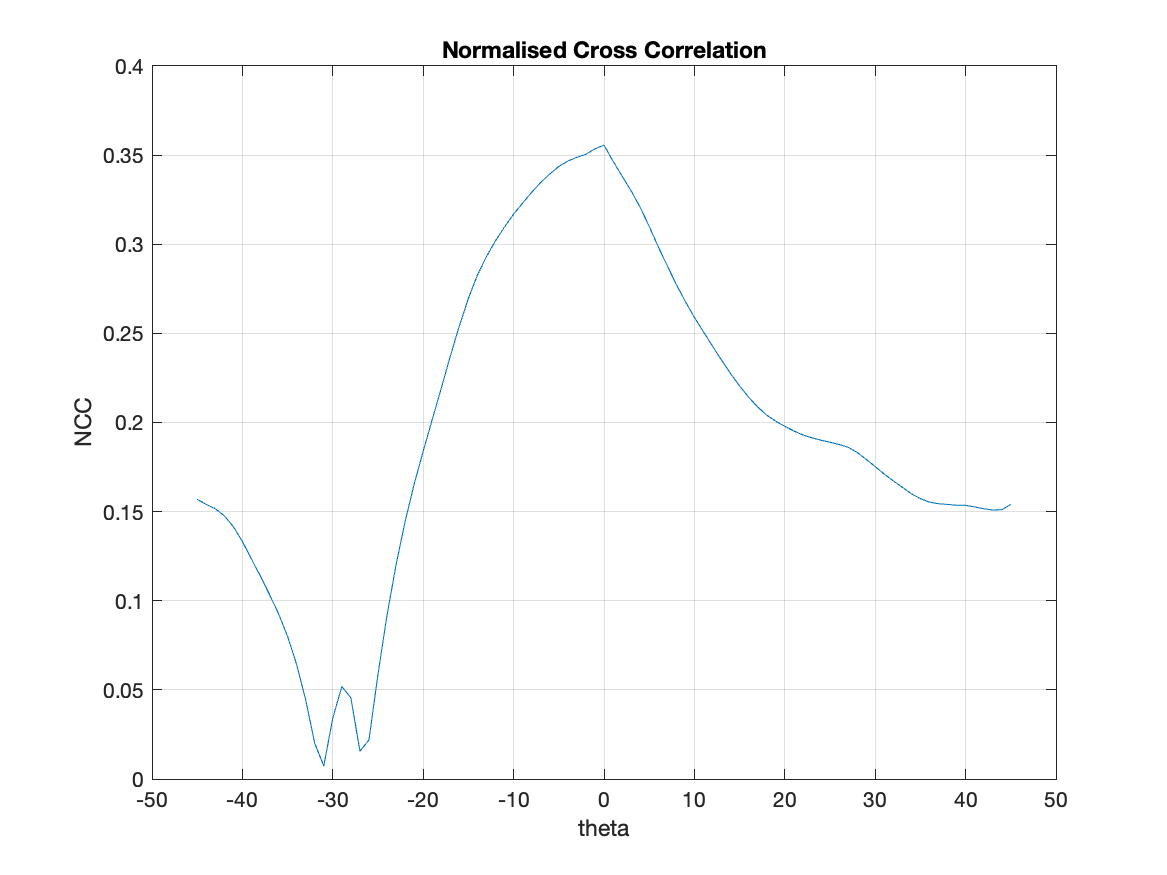
\includegraphics[width=0.59\textwidth]{../images/NCC.png}
        \vspace{-10pt}
        \caption{Normalised Cross Correlation (NCC) v/s $\theta$}
    \end{figure}
    
    \vspace{-25pt}
    
    \begin{figure}[H]
        \centering
        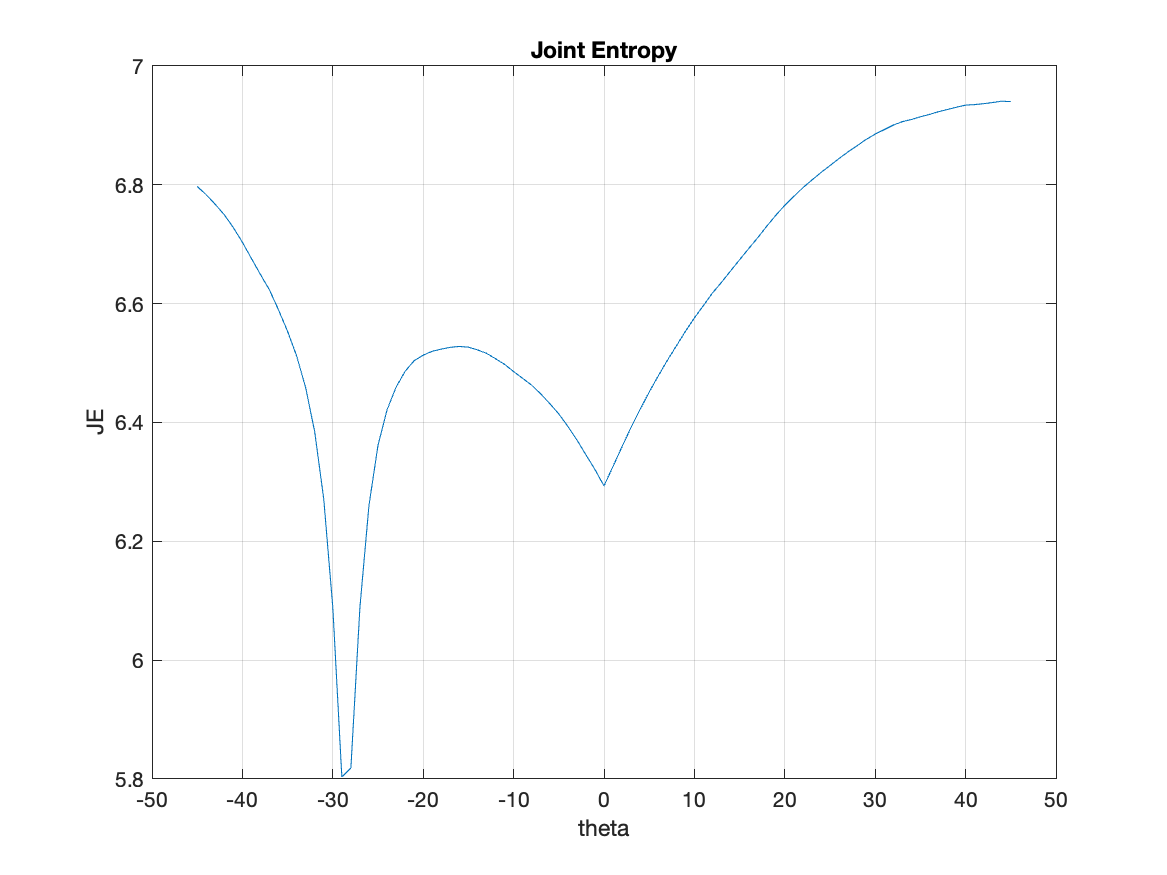
\includegraphics[width=0.59\textwidth]{../images/JE.png}
        \vspace{-10pt}
        \caption{Joint Entropy (JE) v/s $\theta$}
    \end{figure}
    
    \vspace{-25pt}
    
    \begin{figure}[H]
        \centering
        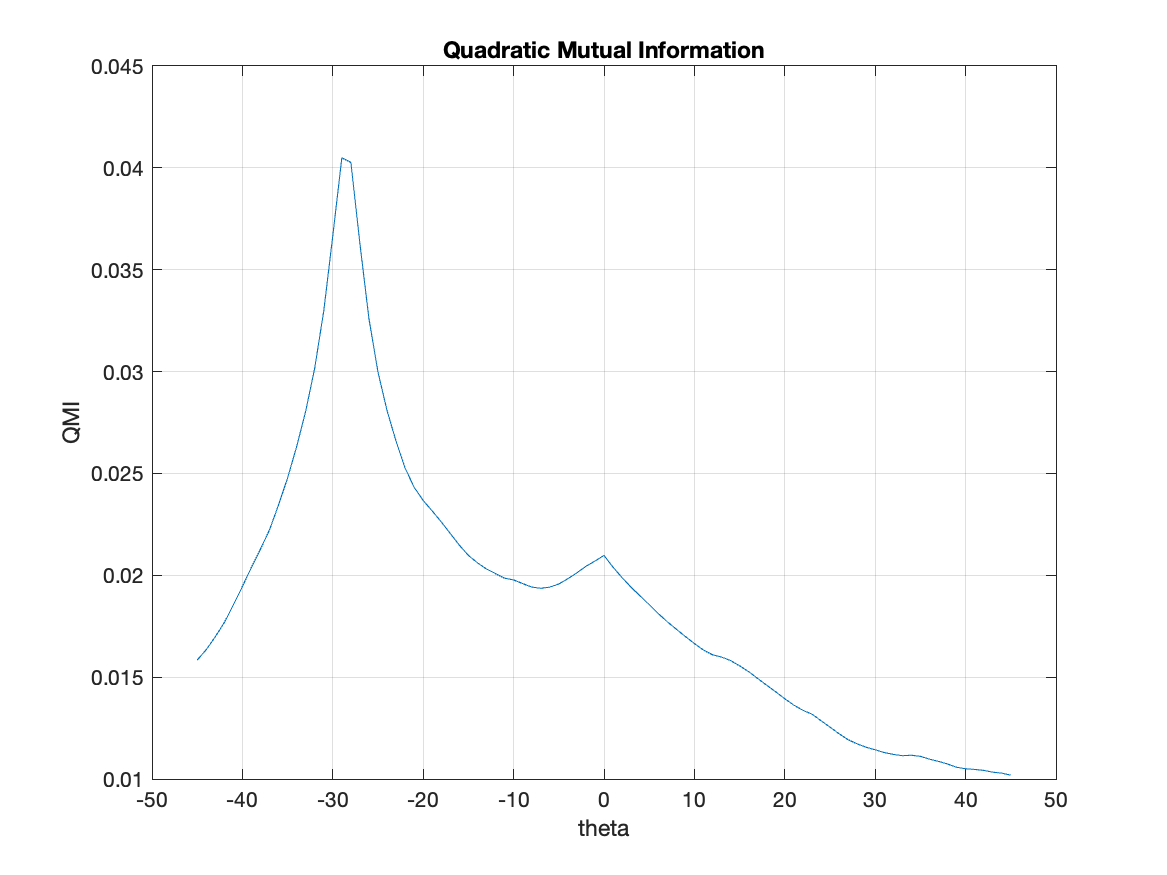
\includegraphics[width=0.59\textwidth]{../images/QMI.png}
        \vspace{-10pt}
        \caption{Quadratic Mutual Information (QMI) v/s $\theta$}
    \end{figure}
    
    \textbf{(d)} Here are some observations:-
    
    \vspace{-10pt}
    
    \begin{itemize}[itemsep=0em]
        \item \textbf{NCC:} More the absolute value of NCC, better the linear relation between the images. Global maxima exists at $\theta = 0^{\circ}$, which is clearly not the correct rotation. There does exist a local maxima at around $\theta = -29^{\circ}$ as expected. Hence it can be observed that NCC is not always a good measure to deal with image alignment.
        \item \textbf{JE:} Lesser the JE, better the alignment. We see that the global minima exists at $\theta = -29^{\circ}$, close to our expected value ($28.5^{\circ}$ clockwise) upto precision of 1 degree, given the step size of theta is 1 degree too. Hence, JE checks out to be a good method for dealing with image alignment. We also observe a local minima at $\theta = 0^{\circ}$.
        \item \textbf{QMI:} More the QMI, better the alignment. We see that the global maxima exists at $\theta = -29^{\circ}$, close to our expected value ($28.5^{\circ}$ clockwise) upto precision of 1 degree, given the step size of theta is 1 degree too. Hence, QMI too checks out to be a good method for dealing with image alignment. We also observe a local maxima at $\theta = 0^{\circ}$.
    \end{itemize}
    
    \vspace{-10pt}
    
    Here are the optimal rotations:-
    
    \vspace{-10pt}
    
    \begin{table}[H]
        \centering
        \begin{tabular}{|c|c|}
            \hline
            Measure & Optimal $\theta$ \\
            \hline
            NCC & $0^{\circ}$ \\
            JE & $-29^{\circ}$ \\
            QMI & $-29^{\circ}$ \\
            \hline
        \end{tabular}
    \end{table}
    
    \vspace{-10pt}
    
    \textbf{(e)} The code is in \texttt{../code/myMainScript.m} and the joint histogram for $\theta = -29^{\circ}$:-
    
    \vspace{-13pt}
    
    \begin{figure}[H]
        \centering
        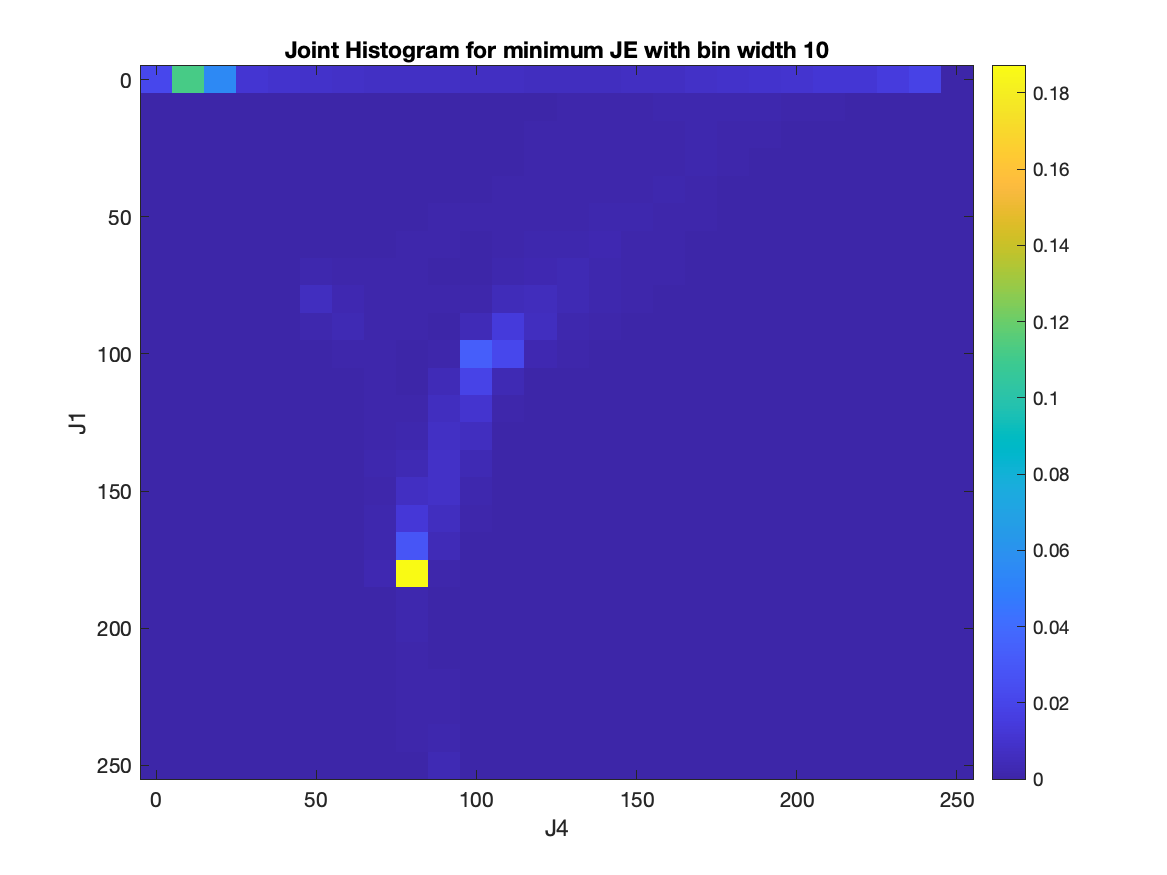
\includegraphics[width=0.59\textwidth]{../images/Joint_hist_JE.png}
        \vspace{-10pt}
        \caption{Joint Histogram for $\theta = -29^{\circ}$}
    \end{figure}
    
    \vspace{-10pt}

    \textbf{(f)} When two discrete random variables $I_1$ and $I_2$ are statistically independent, then $p_{I_1 I_2}(i_1,i_2)=p_{I_1}(i_1) \times p_{I_2}(i_2) \; \forall \; i_1, i_2$ (in domain of the variables), i.e. joint PMF is equal to product of the marginal PMFs. In that case, QMI would be equal to $0$. Hence the more the difference between $p_{I_1 I_2}(i_1,i_2)$ and $p_{I_1}(i_1) \times p_{I_2}(i_2)$, the more dependent the variables are. Hence the more aligned (correlated) the images are, QMI tends to be higher. Hence images are aligned when QMI is maximum.
    
    Also unlike NCC, QMI can detect non-linear relation between variables.
\clearpage
\end{document}